\documentclass[a4paper,10pt]{article}
\usepackage[utf8]{inputenc}
\usepackage{fullpage}
\usepackage[T1]{fontenc}
\usepackage[hidelinks]{hyperref}
\usepackage{graphicx}

\setlength{\parskip}{0.4\baselineskip}
\setlength{\parindent}{0cm}

\begin{document}
\title{Process book: DataMoviz}
\author{Quentin de Longraye, Aymen Gannouni, Victor Le}

\maketitle

\begin{figure}[ht]
   \centering
   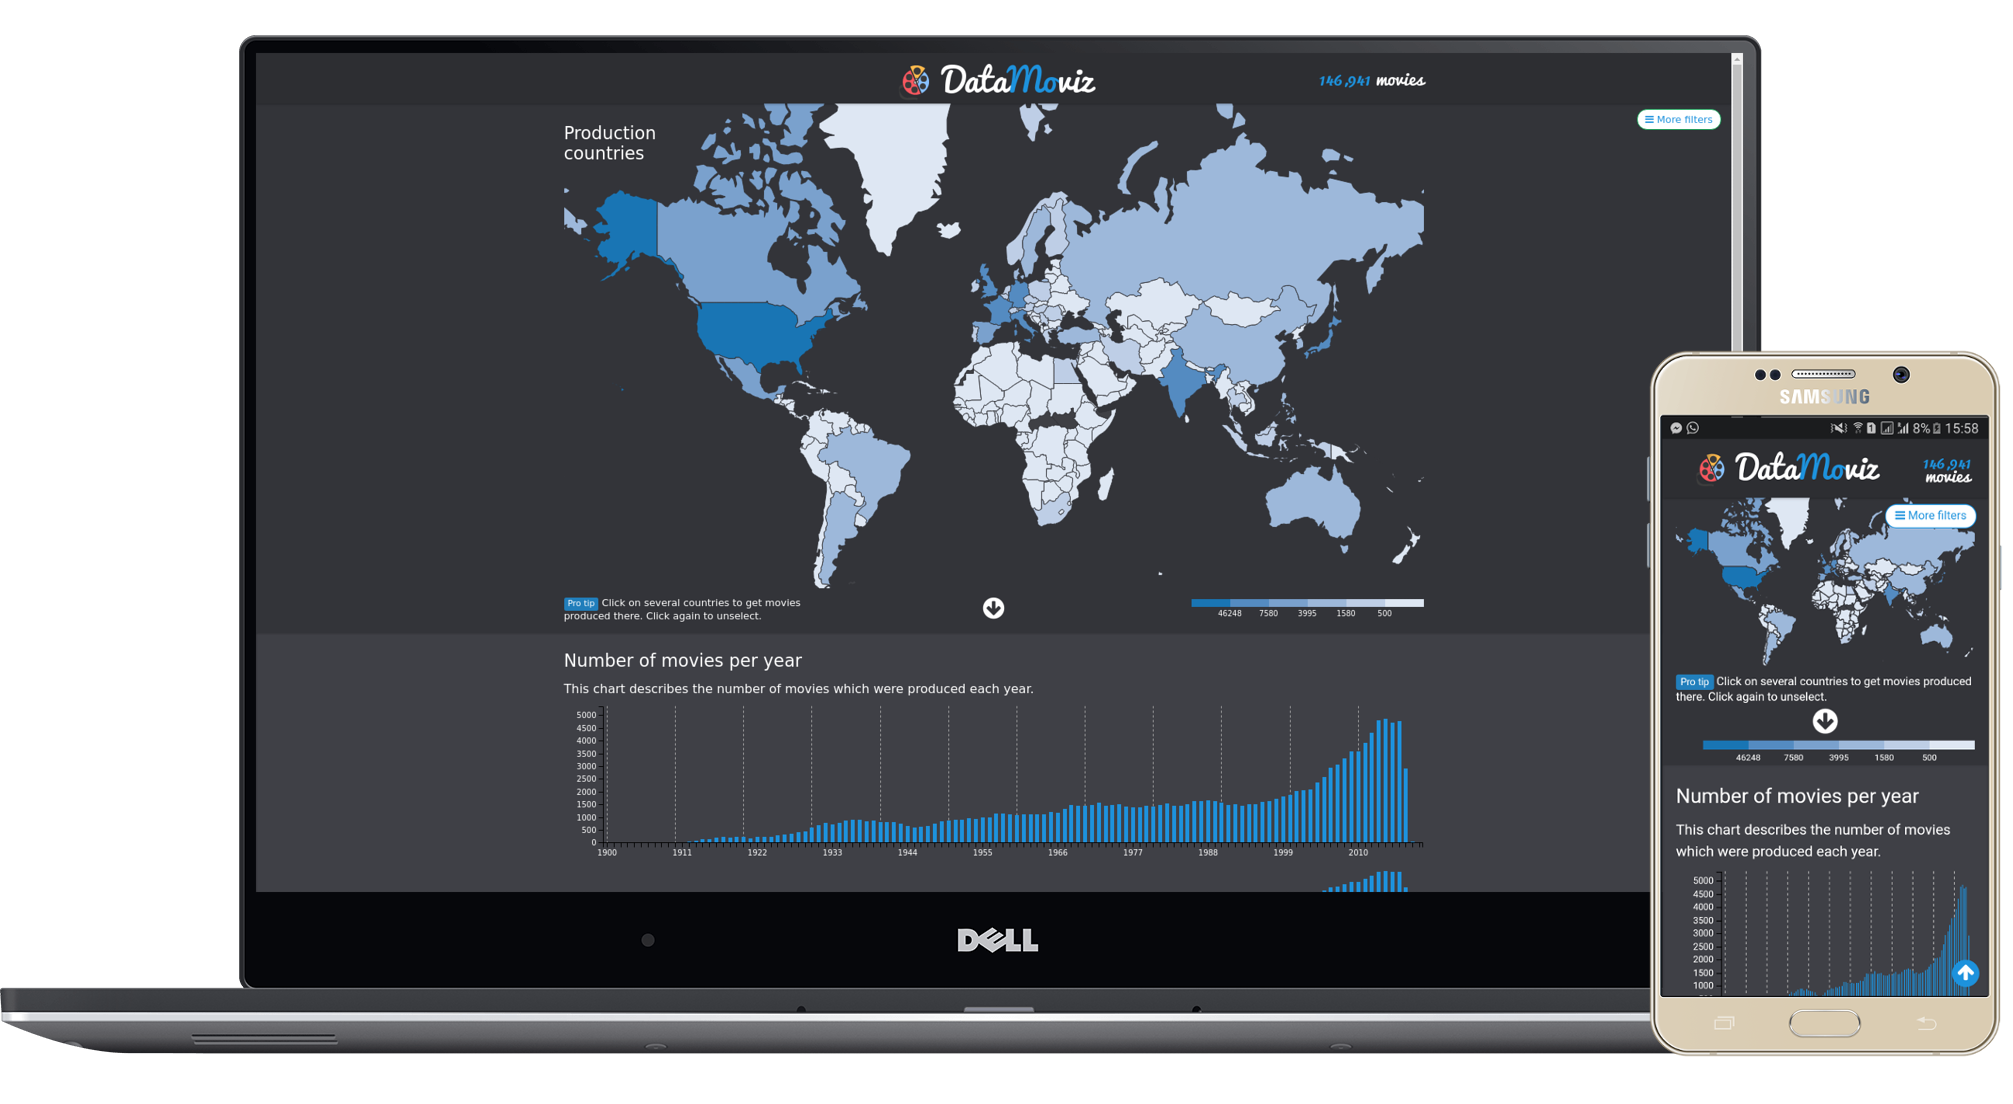
\includegraphics[width=1\linewidth]{../docs/mockup.png}
  \caption{Datamoviz mockup}
\end{figure}

\setlength{\parskip}{0.1\baselineskip}

\tableofcontents

\setlength{\parskip}{0.4\baselineskip}

\newpage

\section{Presentation of DataMoviz}

\subsection{Overview, motivation and target audience}
Overview, motivation, target audience
+ Questions: What am I trying to show this my viz?

DataMoviz is a web application, that aims at involving the user in a unique experience to discover all the movies from The Movie Database in a very interactive way. This project allows to get impressive insights on the filmmaking scence scince the beginnings.
What motivates us the most is the opportunity that we have to deliver fascinating observations from raw data through data visualization.
There is no restrictions in term of prerequisites for our target audience. Anyone who has interest in movies is heartly welcomed to visit DataMoviz!

\subsection{Related work and inspiration}

Related work and inspiration

\section{Exploratory analysis}

\subsection{Dataset}

Presentation of the dataset.
Dataset: where does it come from, what are you processing steps?

\subsection{Data previsualization}

Exploratory data analysis: What viz have you used to gain insights on the data?

\section{Solution's build-up}

\subsection{Considered visualizations}

Designs: What are the different visualizations you considered? Justify the design decisions you made using the perceptual and design principles.
Did you deviate from your initial proposal?

\subsection{Implementation}

Implementation: Describe the intent and functionality of the interactive visualizations you implemented. Provide clear and well-referenced images showing the key design and interaction elements.

\subsubsection{Presentation of the visualizations}

In the section, we will present each visualizations and the insights it brings about
the data.

\paragraph{The filters bar and panel} The filter panel allows user to see which filters are
currently applied on page's data (fig. \ref{fig:filters-bar}). It permits to give an explicit explanation about
page current's sate. Users are allowed to remove a filter by clicking on the small
cross near the filter description. They can also click on \textit{more filters} to
have access to three more page filters: filtering by keywords in movie titles,
by genre and by content rating.

\begin{figure}[ht]
  \centering
  
\includegraphics[width=1\linewidth]{images/screens/filters-bar-example.png}
  \caption{The filters bar with applied filters} \label{fig:filters-bar}
\end{figure}

\paragraph{The interactive map} The interactive map is the first visible visualization
when going into the DataMoviz website. This visualization allows to understand which
countries are more involved into producing movies, considering all the applied filters
by other application components (see section \ref{sec:filtering-system} for more details).
When the user selects a country, the maps colors changes smoothly to let the user understand
the transition between the two states (unfiltered to filtered state). The figure \ref{fig:country-selection}
shows what happened after selecting a country (here, we click on France).

\begin{figure}[ht]
  \centering
  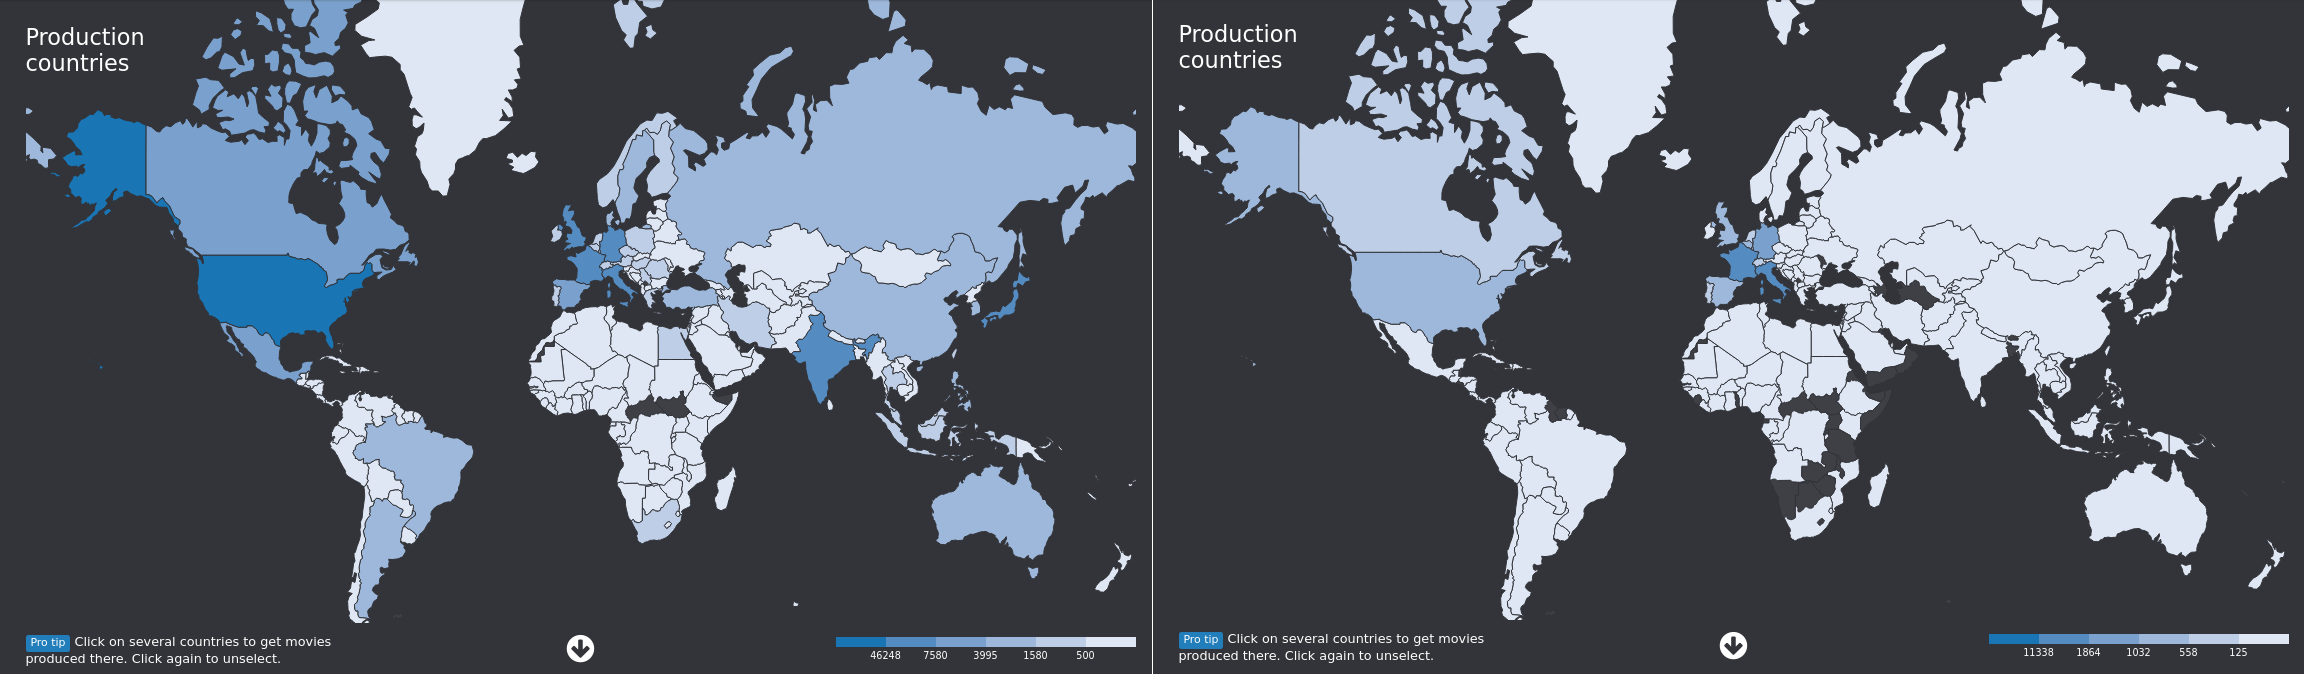
\includegraphics[width=1\linewidth]{images/screens/country-selection.png}
  \caption{Initial draft of the filtering system} \label{fig:country-selection}
\end{figure}

As we can see, all colors intensity decreases. We still have a lot of colored countries
because all of them participated into the production of some movies together with
french production companies. The color intensity allows the user to understand which
countries were more involved in movie production based on current filters, but also
which countries co-producted movies with France the most (here: Italy and Germany).

\paragraph{The time evolution}

The second visualization is a time evolution display and selector. It allows to
see how the number of produced movies evolved over time, considering the selected
filters. Users can interact with this visualization by selecting a time range in the
subchart (fig. \ref{fig:time-selection}). This will create a new filter and restrict all gathered data for a specific
time range. All the other visualizations will be updated consequently.

\begin{figure}[ht]
  \centering
  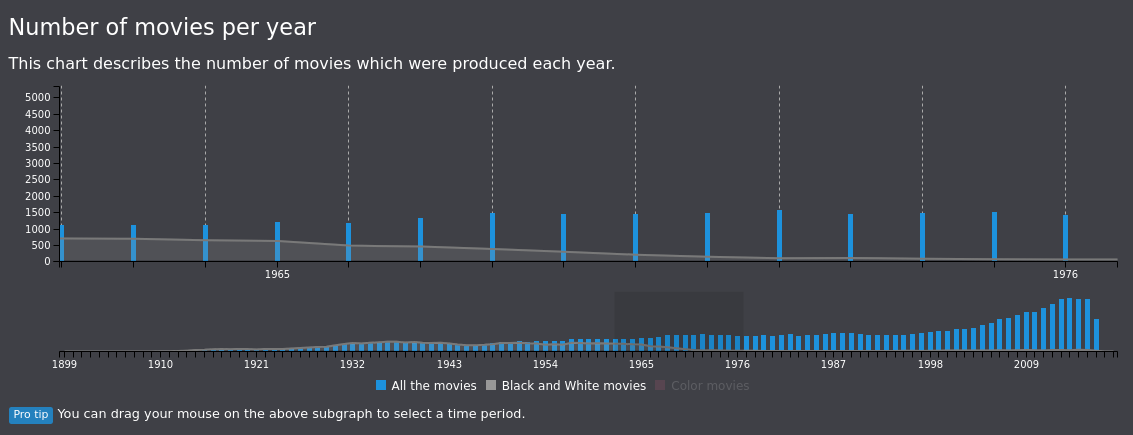
\includegraphics[width=1\linewidth]{images/screens/time-selection.png}
  \caption{The time evolution with 1970-1985 period selected} \label{fig:time-selection}
\end{figure}

In figure \ref{fig:time-selection}, we can see that black and white movies were
also selected. This allows to see how black and white movie distribution evolved
for the time range.



\paragraph{The actors network}
The actor network is a vizualization that shows how the movies are related.
The relation is based on the shared crew members. Each movie and actor are represented as
a node in the graph. The color of this one indicates its genre or role respectively.
A edge is defined between two movies if and only if there is at least one actor who
plays in both of them. Its width is correlated to the number of actor in common.
By default, the graph only shows the movies : to show the crew who plays for one,
we can just click on the corresponding node.

\begin{figure}[ht]
   \centering
   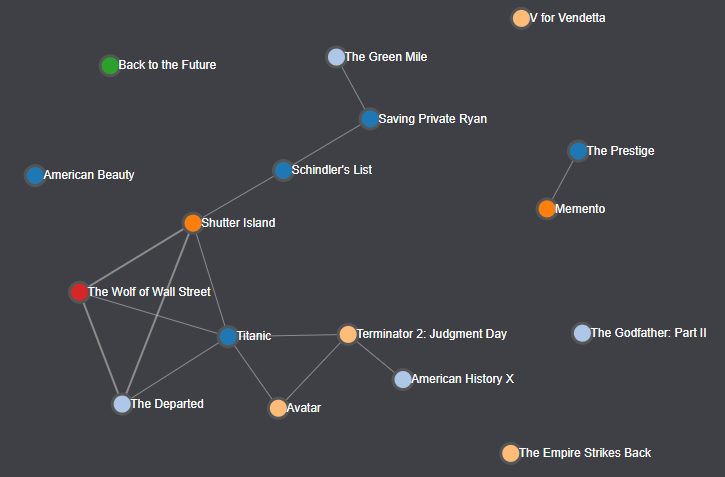
\includegraphics[width=0.6\linewidth]{images/screens/network-movies.png}
  \caption{The network} \label{fig:screen-network-movies}
\end{figure}

\begin{figure}[ht]
   \centering
   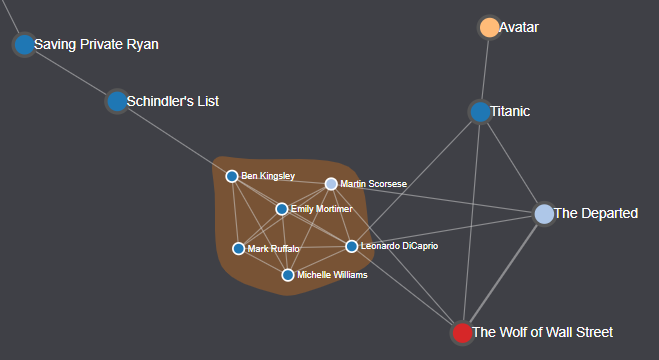
\includegraphics[width=0.6\linewidth]{images/screens/network-movies-shutter-island.png}
  \caption{The network with Shutter Island actors} \label{fig:screen-network-movies-shutter-island}
\end{figure}

The network is highly interactive and customizable. We can change the number of actors,
crew members and movies to show thanks to some sliders. SHOW PICTURE.
This vizualization offers a way to navigate freely through the network : it supports panning,
and zooming. If the user got lost, he can reset easily to default zoom by pressing a button, no
need to reload the page. Moreover, if we are not interested to having the movies name and actors name shown,
we can turn it off. Anyway, a hover on a node shows this information in addition to
indicating the role or genre respectively for actors and movies.

\begin{figure}[ht]
   \centering
   
\includegraphics[width=0.6\linewidth]{images/screens/network-movies-checkboxes.png}
  \caption{The checkboxes} \label{fig:screen-network-movies-checkboxes}
\end{figure}

\begin{figure}[ht]
   \centering
   
\includegraphics[width=0.6\linewidth]{images/screens/network-movies-sliders.png}
  \caption{The sliders} \label{fig:screen-network-movies-sliders}
\end{figure}


\subsubsection{The filtering system} \label{sec:filtering-system}

The filtering system is one of the most important features of this visualization.
It allows to interact with the page and asserts all graphs are in the same, coherent
state. Without this system, we would not have been able to provide an visually interactive web application.
It was built by creating a single shared state between all components. Each
time a component needs to update the filters, it triggers an event which is relayed
to the other components. The following draft (fig. \ref{fig:draft-filtering}) describes how the system works. It
was designed before implementation.

\begin{figure}[ht]
   \centering
   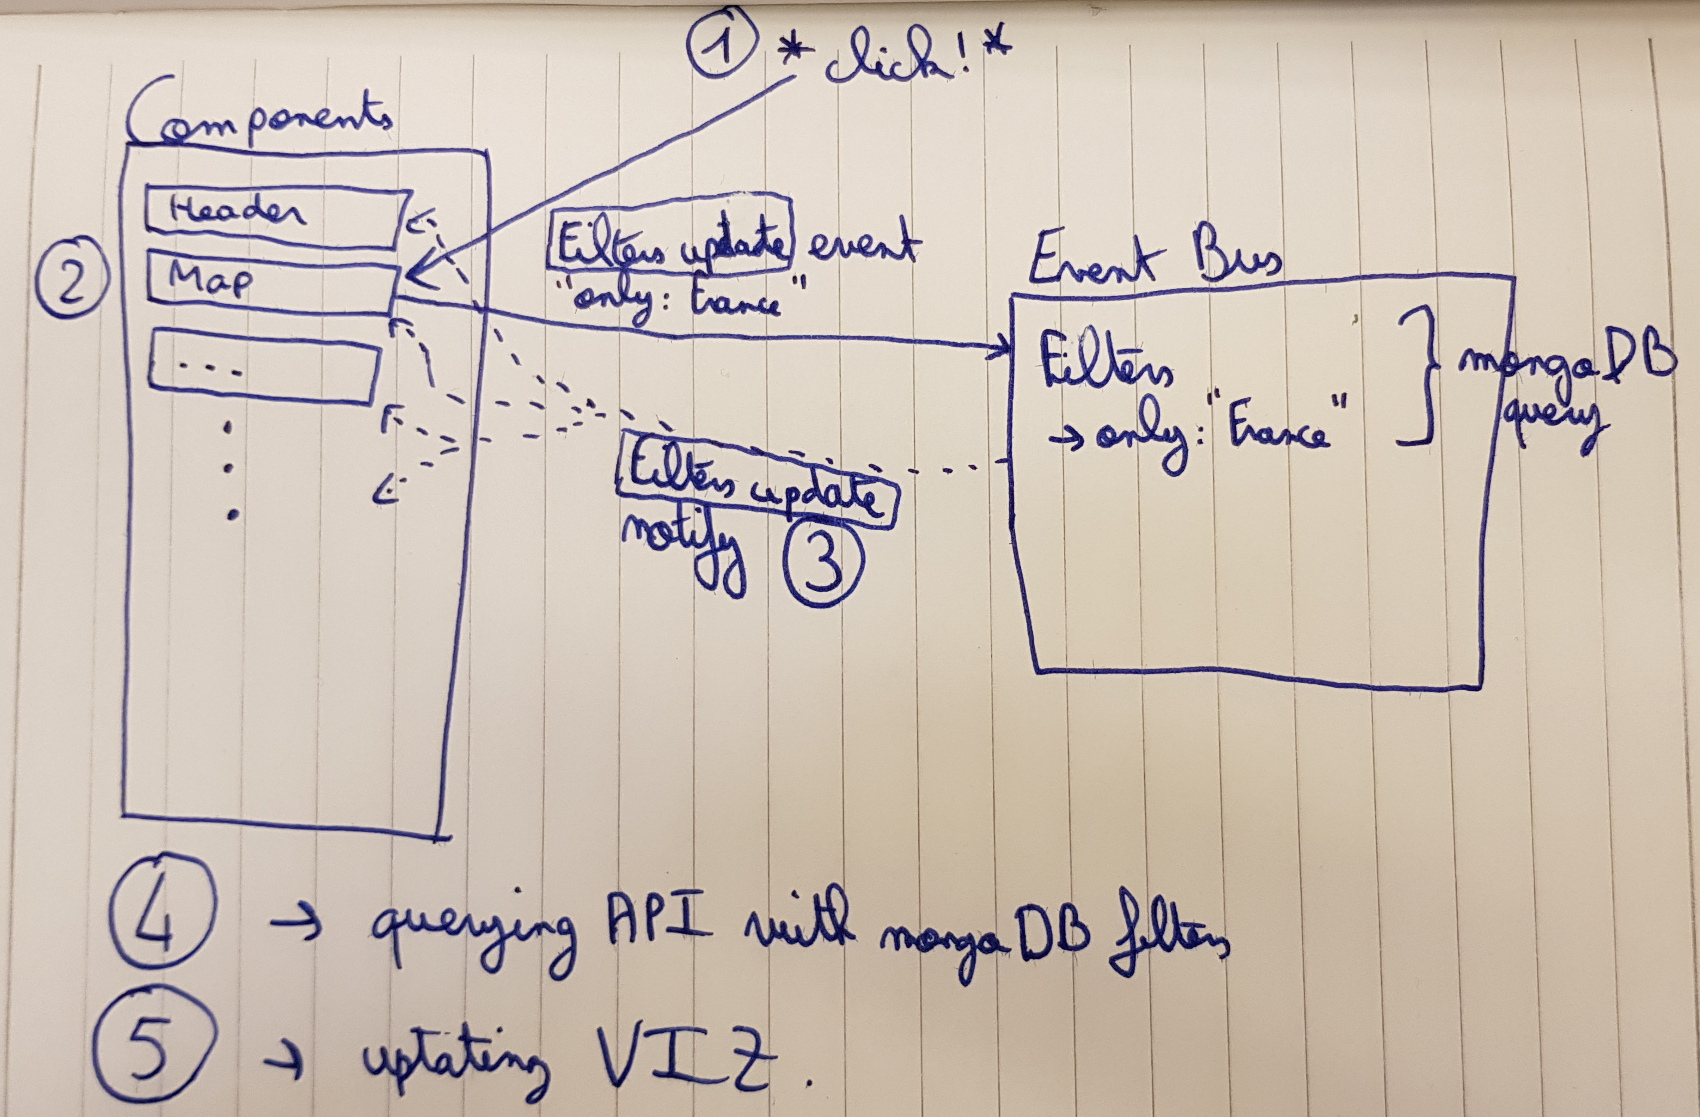
\includegraphics[width=0.6\linewidth]{images/drafts/filtering-system.jpg}
  \caption{Initial draft of the filtering system} \label{fig:draft-filtering}
\end{figure}

When the user interacts with the page (for instance by clicking on a country of the
map visualization (1)), a filters update event is triggered into an event bus (2). This
event contains all the filters that are currently applied to get the data for each
component of the application, with a small addition or deletion (the example shows
a constraint in which the user wants to filter to get only movies produced in France).
The event bus redirects this filter to all the subscribed components (3). Based on
the new filters, they may query the API (4) to get refreshed data, and can update
the visualization consequently (5).

This system was designed following simple computational thinking concepts, by reducing
the filtering complexity into a single, atomic and context-independent (stateless) set of filters which can be directly
passed to MongoDB to filter data. We also take leverage of HTTP cache to allow
the browser to cache all previous requests, so we potentially avoid overwhelming processing
on the server.

The final implementation is presented in the figure \ref{fig:screen-filtering}.
This event happened after clicking on France country. We can see in the event
payload that an object is stored. This object describes a MongoDB filtering subquery
which may be used by the server to restrict which data should be used during data
selection, aggregation or counting.

\begin{figure}[ht]
   \centering
   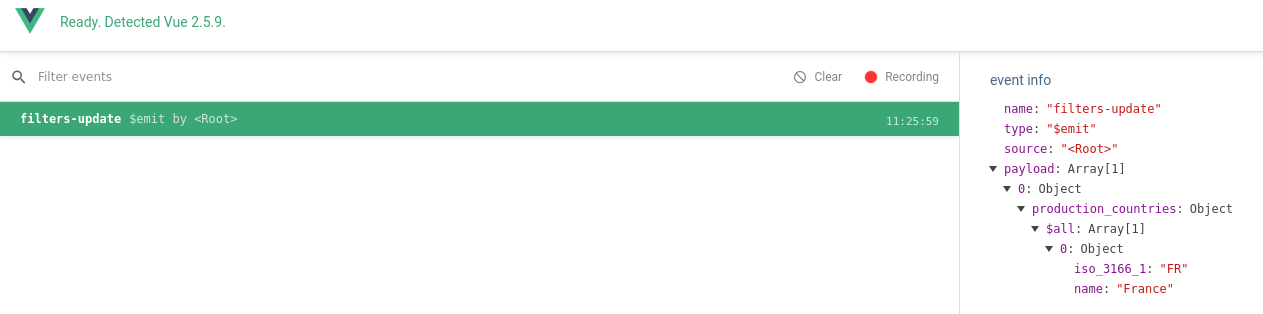
\includegraphics[width=1\linewidth]{images/screens/filtering-example.png}
  \caption{An emitted event when selecting a country} \label{fig:screen-filtering}
\end{figure}

This system is extremely flexible as it allows to add new components without impacting
other parts of the application. Each new component should only define two behaviors (if required):
filters update triggering after user interaction, and filters update handling when
another component udpates the filters.

\subsection{Evaluation}

Evaluation: What did you learn about the data by using your visualizations? How did you answer your questions? How well does your visualization work, and how could you further improve it?

\section{Peer assessment}

\begin{itemize}
  \item Preparation – were they prepared during team meetings?
  \item Contribution – did they contribute productively to the team discussion and work?
  \item Respect for others’ ideas – did they encourage others to contribute their ideas?
  \item Flexibility – were they flexible when disagreements occurred?
\end{itemize}

\setlength{\parskip}{0.1\baselineskip}

\newpage

\listoffigures

\end{document}
